\documentclass[twocolumn,twoside]{article}

% Modified Template by Jonathan Doucette and Kevin Multani, original by: Jonathan Ward

\documentclass[12pt]{article} 
\usepackage[english]{babel}
\usepackage[utf8]{inputenc}
\usepackage{amsmath} % AMS Math Package
\usepackage{amsthm} % Theorem Formatting
\usepackage{amssymb} % Math symbols such as \mathbb
\usepackage{graphicx} % Allows for eps images
\usepackage{multicol} % Allows for multiple columns
\usepackage[dvips,letterpaper,margin=1in,bottom=1in]{geometry}
\usepackage{hyperref}
\usepackage{parskip} % Removes indentation from paragraphs
\usepackage{xcolor,xspace,soul} % Colour, spacing, and highlighting
\usepackage{mathrsfs}
\usepackage{bm} % For bold math symbols
\usepackage{amscd}
\usepackage[all,cmtip]{xy}
%\usepackage{bbm}
\usepackage{titling}
\usepackage{listing} % for code snippets
%\usepackage{minted} % for code snippets
\usepackage{enumerate}
\usepackage{fancyhdr}
\usepackage[]{physics}
\usepackage[makeroom]{cancel}
\usepackage{pdfpages}
\usepackage[]{mcode}
\usepackage[title]{appendix}

% ***********************************************************
% ********************** BEGIN TITLE PAGE *******************
% ***********************************************************
\newcommand*{\titleGM}{\begingroup % Create the command for including the title page in the document
\hbox{ % Horizontal box
\hspace*{0.2\textwidth} % Whitespace to the left of the title page
\rule{1pt}{\textheight} % Vertical line
\hspace*{0.05\textwidth} % Whitespace between the vertical line and title page text
\parbox[b]{0.75\textwidth}{ % Paragraph box which restricts text to less than the width of the page

{\noindent\Huge\bfseries MATH 521}\\[2\baselineskip] % Title
{\large \textit{Assignment 4}}\\[4\baselineskip]
%{\large \textsc{ Jonathan Doucette }} % Author name

\vspace{0.5\textheight} % Whitespace between the title block and the publisher
{\noindent \today }\\[\baselineskip]
%{\noindent Student Number: 35298124 }\\[\baselineskip] 
%{\noindent \footnotesize All problems below are \textit{Copyright \copyright \space 2018 Timm Treskatis. All Rights Reserved.} }\\[\baselineskip]
} % end parbox
} % end hbox
\endgroup}

 % Sets margins and page size
\pagestyle{fancy} 

%\lhead{Jonathan Doucette}
\rhead{\today}
\rfoot{Page \thepage}
\cfoot{}

\makeatletter % Need for anything that contains an @ command 
\renewcommand{\maketitle} % Redefine maketitle to conserve space
{ \begingroup \vskip 10pt \begin{center} \Huge {\bf \@title}
\vskip 10pt \large \@author \hskip 20pt \@date \end{center}
  \vskip 10pt \endgroup \setcounter{footnote}{0} }
\makeatother % End of region containing @ commands

% ***********************************************************
% ********************** END TITLE PAGE *********************
% ***********************************************************

% ***********************************************************
% ********************** BEGIN NEW COMMANDS *****************
% ***********************************************************

\renewcommand{\labelenumi}{(\alph{enumi})} % Use letters for enumerate
\let\vaccent=\v % rename builtin command \v{} to \vaccent{}

%% MISC
\newcommand{\ab}[1]{\left| #1 \right|} % for absolute value
\newcommand{\avg}[1]{\left< #1 \right>} % for average
\let\underdot=\d % rename builtin command \d{} to \underdot{}
\let\baraccent=\= % rename builtin command \= to \baraccent
\renewcommand{\=}[1]{\stackrel{#1}{=}} % for putting numbers above =
\providecommand{\fr}{\frac}
\providecommand{\RR}{\mathbb{R}}
\providecommand{\CC}{\mathbb{C}}
\providecommand{\NN}{\mathbb{N}}
\providecommand{\e}{\epsilon}
\DeclareMathOperator{\di}{d\!}
\newcommand*\ieval[3]{\left.#1\right\rvert_{#2}^{#3}}

%% Vectors
\renewcommand{\v}[1]{\ensuremath{\mathbf{#1}}} 
\newcommand{\gv}[1]{\ensuremath{\mbox{\boldmath$ #1 $}}} % for vectors of Greek letters
\newcommand{\uv}[1]{\ensuremath{\mathbf{\hat{#1}}}} % for unit vector
\providecommand{\wave}[1]{\v{\tilde{#1}}}

%% DERIVATIVES
\renewcommand{\d}[2]{\frac{d #1}{d #2}} % for derivatives
\newcommand{\dubd}[2]{\frac{d^2 #1}{d #2^2}} % for double derivatives
\newcommand{\pd}[2]{\frac{\partial #1}{\partial #2}} % for partial derivatives
\newcommand{\pdd}[2]{\frac{\partial^2 #1}{\partial #2^2}} % for double partial derivatives

%% Operators
\newcommand{\Gradient}{\ensuremath{\mbox{\boldmath$\nabla$}}} % gradient

%% Text
\newcommand{\mathcolorbox}[2]{\colorbox{#1}{$\displaystyle #2$}}
\newcommand{\hlfancy}[3]{\textcolor{#1}{\sethlcolor{#2}\hl{#3}}}
\newcommand{\TODO}[1]{\hlfancy{red}{yellow}{\textbf{TODO: #1}}}

%% Code
%\newcommand{\code}[1]{\mintinline{C}{#1}}
%\newcommand{\code}[1]{\texttt{#1}}
\newcommand{\code}[1]{\lstinline[columns=fixed]{#1}}
\newcommand{\includecode}[1]{\lstinputlisting{#1}}

% ***********************************************************
% ********************** END NEW COMMANDS *******************
% ***********************************************************

% ***********************************************************
% ********************** BEGIN NEW ENVS *********************
% ***********************************************************

% Theorem
\newenvironment{theorem}[2][Theorem]{\begin{trivlist}
\item[\hskip \labelsep {\bfseries #1}\hskip \labelsep {\bfseries #2.}]}{\end{trivlist}}
% Lemma
\newenvironment{lemma}[2][Lemma]{\begin{trivlist}
\item[\hskip \labelsep {\bfseries #1}\hskip \labelsep {\bfseries #2.}]}{\end{trivlist}}
% Corollary
\newenvironment{corollary}[2][Corollary]{\begin{trivlist}
\item[\hskip \labelsep {\bfseries #1}\hskip \labelsep {\bfseries #2.}]}{\end{trivlist}}

% Exercise
\newenvironment{exercise}[2][Exercise]{\begin{trivlist}
\item[\hskip \labelsep {\bfseries #1}\hskip \labelsep {\bfseries #2.}]}{\end{trivlist}}
% Problem
\newenvironment{problem}[2][Problem]{\begin{trivlist}
\item[\hskip \labelsep {\bfseries #1}\hskip \labelsep {\bfseries #2.}]}{\end{trivlist}}
% Question
\newenvironment{question}[2][Question]{\begin{trivlist}
\item[\hskip \labelsep {\bfseries #1}\hskip \labelsep {\bfseries #2.}]}{\end{trivlist}}
% Solution
\newenvironment{solution}{\begin{proof}[Solution]}{\end{proof}}

% Afterword
\newenvironment{afterword}[2][Appendix]{\begin{trivlist}
\item[\hskip \labelsep {\bfseries #1}\hskip \labelsep {\bfseries #2}]}{\end{trivlist}}

% ***********************************************************
% ********************** END NEW ENVS ***********************
% ***********************************************************

% ***********************************************************
% ********************** END TITLEPAGE **********************
% ***********************************************************

%% ------------------------------------------------------ %%
%% ----------------------- Title ------------------------ %%
%% ------------------------------------------------------ %%

\setlength{\droptitle}{-0.5cm}
\title{Numerical Methods in Magnetic Resonance Imaging:\\The Bloch-Torrey Equation\vspace{0.3cm}}

\author[a,b]{Jonathan Doucette}

\affil[a]{UBC MRI Research Centre, University of British Columbia,
  2221 Wesbrook Mall, Vancouver, BC, Canada.}

\affil[b]{Department of Physics and Astronomy, University of British
  Columbia, 6224 Agricultural Road, Vancouver, BC, Canada.\vspace{0.3cm}}

\date{\today}
\setcounter{Maxaffil}{0}
\renewcommand\Affilfont{\itshape\small}

\begin{document}

\maketitle

%Corresponding author footer
\let\thefootnote\relax\footnote{e-mail: \texttt{jdoucette@phas.ubc.ca}}
%{\let\thefootnote\relax\footnote{{\textsuperscript{†}e-mail: jdoucette@phas.ubc.ca}}}

%TODO Abstract
\vspace{-0.63cm}
\textbf{In magnetic resonance imaging, insight into different imaging modalities can be gained through the simulation of the magnetic resonance signal measured by the scanner.
This signal is modelled as the solution of the parabolic Bloch-Torrey partial differential equation.
In this work, I compare various numerical techniques for solving the Bloch-Torrey equation in the presence of highly discontinuous data with the goal of optimising the trade-off between solution accuracy and computation time.}

\section*{Introduction}
In magnetic resonance imaging (MRI), insight into different imaging modalities can be gained through the simulation of the magnetic resonance (MR) signal from first principles.
The MR signal which is measured by an MRI scanner within a given region  is directly proportional to the magnitude of the net magnetization vector \MM{} within that region.
In tissue, \MM{} arises due to the superposition of the magnetic moments of water molecules, also known as \textit{spins} in MRI nomenclature.
Ordinarily, \MM{} is zero in tissue as spins are randomly oriented and therefore their vector sum is zero on the average.
In MRI, however, there is a large and constant external magnetic field $\v{B_0} = B_0 \uv{z}$ which forces the alignment of the magnetized spins with $\v{B_0}$, taken here to be along the $z$-direction.
This allows for the measurement, and importantly, the manipulation of the otherwise negligible net magnetization \MM{} of the spins.

In one common type of MRI scan, a \textit{gradient echo} scan, \MM{} is initially flipped into the $xy$-plane through the application of a radio frequency (RF) magnetic pulse.
Immediately, \MM{} begins to realign with $\v{B_0}$ exponentially quickly.
The rate \rr{} at which this realignment occurs, however, depends on local tissue properties. % and therefore the realignment occurs at different rates at different locations in space.
Additionally, there is a characteristic precession of \MM{} about $\v{B_0}$ as it realigns.
This precession occurs at a rate \ww{} which, too, depends on the magnetic properties of the environment.
Lastly, spins are free to diffuse within their environment while realigning, which means that they will see varying \rr{} and \ww{} as they move through the tissue.

\subsection*{The Bloch-Torrey equation}

In the continuum limit, the net magnetization \MM{} within a given region is modelled as a continuous vector field, and the complex dynamics which follow the initial RF pulse can be beautifully modelled as solutions to a parabolic partial differential equation (PDE) called the Bloch-Torrey equation~\cite{torrey_bloch_1956}:
%
\begin{equation}\label{BTreal}
\begin{cases}
\ddt{u} = D \Laplacian{u} - R u + \omega v\\%, \qquad u(\v{x},0) = M_x(\v{x},0) \\
\hspace{0.5pt}\ddt{v} = D \Laplacian{v} - R v - \omega u\\%, \qquad \hspace{1pt} v(\v{x},0) = M_y(\v{x},0).
\end{cases}
\end{equation}
%
Here, $u$ and $v$ are the $x$- and $y$-components of the magnetization \MM{} and $D$ is the diffusion constant.
For short simulation times, or \textit{echo times}, $T$, the $z$-component of \MM{} does not change appreciably, and we need only consider the transverse magnetization $\Mt{} = (u,v)$.

The transverse Bloch-Torrey equation~\eqref{BTreal} may be equivalently written as
%
\begin{equation}\label{BTcplx}
\ddt{\Mxy} = D \Laplacian{\Mxy} - \CDecay \Mxy
\end{equation}
%
where $\Mxy = u + i v$ is the complex magnetization and $\CDecay(\v{x}) = R(\v{x}) + i \omega(\v{x})$ is the complex decay rate.
This form is both notationally convenient and conceptually illustrative; now, realignment with \Bo{} corresponds to the magnitude of the (complex) transverse magnetization $\Mxy$ decaying to zero, and the precession of \MM{} about \Bo{} corresponds to the rotation of $\Mxy$ about the origin in the complex plane.

\subsection*{Signal simulation}
This work will compare three different methods of simulating the signal $S(T)$ measured by an MRI scanner at a time $T$ following an initial RF pulse: finite differences, splitting methods, and finite element methods.

The MR signal $S(T)$ is given by
%
\begin{equation}
S(T) = \Norm{\int_\Omega \Mt{}(T) \dx{x}}
\end{equation}
%
where $\Mt{}(T)$ is computed by solving~\eqref{BTreal} or~\eqref{BTcplx}. The initial transverse magnetization $\Mt{}(t=0)$ will be taken to be $[0,1]^T$ without loss of generality.%, noting that multiplying~\eqref{BTcplx} by a complex constant $\alpha$ simply results in a final signal which is scaled by $\ab{\alpha}$.

\subsection*{Geometry}
The transverse magnetization $\Mt{}$ will be simulated within a cubic domain $\Omega$ of size $3\times3\times\SI{3}{mm^3}$ with a single cylinder of a variable radius $a$ in the centre of the domain, as pictured in Figure~\ref{fig:geometry}.

This geometry is chosen for two reasons.
First, biologically it represents a single vessel present within a cubic imaging voxel.
Second, there exists an exact solution for \ww{} given the magnetic susceptibility $\chi$ of the cylindrical blood vessel.
For a cylinder of radius $a$, we have that
%
\begin{equation}\label{omega}
\ww{} = 
\begin{cases}
\frac{\chi B_0}{2}\sin^2\theta \frac{a^2}{x^2+y^2} \frac{y^2-x^2}{x^2+y^2}, \hspace{0.2cm} \text{inside cylinder}\\%x^2 + y^2 \geq a^2 \\
\frac{\chi B_0}{6} \left(3\cos^2\theta - 1\right), \qquad \text{outside cylinder}\\%x^2 + y^2 < a^2
\end{cases}
\end{equation}
%
where $\theta$ is the angle between the cylinder axis and \Bo{}.
An example cross section of \ww{} can be seen in Figure~\ref{fig:geometry}.

\section*{Methods}
Finite difference methods, splitting methods, and finite element methods will be investigated.
First, some basic properties of the Bloch-Torrey equation are described.

\subsection*{Static solution}

If $D = 0$, solutions to~\eqref{BTcplx} are simply complex exponentials
\begin{equation}
\Mxy(\v{x},t) = \Mxy_0 e^{-\CDecay(\v{x}) t} \\
= \left(e^{-\rr{} t} \ab{\Mxy_0}\right) e^{i(\phi_0 - \ww{} t)},
\end{equation}
where we have written $\Mxy_0 = \ab{\Mxy_0} e^{i\phi_0}$ in polar form.
In this form, it is clear to see that the magnitude $\ab{\Mxy} = \Norm{\Mt{}}$ of the transverse magnetization is exponentially damped at rate \rr{} and that the initial phase $\phi_0$ changes at the constant rate \ww{}, which can be interpreted as the transverse magnetization rotating about \Bo{} at a constant angular velocity at each point in space.

\subsection*{Relation to the heat equation}
If $\CDecay = 0$, then~\eqref{BTreal} reduces to two uncoupled heat equations in the transverse magnetization components $u$ and $v$.
This is equivalent to the limit as the magnetic field $B_0 \rightarrow 0$, as the magnetic moments of the spins are not forced to realign with an external field and instead are free to diffuse unhindered.

Mathematically, we should expect that solutions to the Bloch-Torrey equation exhibit some of the same properties as solutions of the heat equation, such as exponential suppression of eigenmodes corresponding to large negative eigenvalues.

\subsection*{Positive definiteness}

The coupled system of PDEs~\eqref{BTreal} can be written as
\begin{align}\label{BTvec}
\begin{cases}
\ddt{\uu{}} = -A \uu{} \quad\text{ in }\Omega,\quad t>0 \\
\uu{}_0 = \v{g} \qquad\hspace{5.5pt} \text{ in }\Omega
\end{cases}
\end{align}
where $\uu{} = [u,v]^T$, zero Neumann conditions are taken on the boundary $\partial\Omega$, and
\begin{align}
    A = \begin{pmatrix}
    -D \Laplacian{} + R & -\omega \\ 
    \omega & -D \Laplacian{} + R
    \end{pmatrix}.
\end{align}
The operator $A$, although asymmetric, is positive definite as
\begin{align*}
\langle \uu{}, A \uu{} \rangle
&= \int_\Omega -D u \Laplacian{u} + R u^2 - D v \Laplacian{v} + R v^2 \dx{x} \\
&= \int_\Omega D \, (||\nabla u||^2 + ||\nabla v||^2) + R \, (u^2 + v^2) \dx{x} \\
&\geq 0 \quad \text{(} >0 \text{ for } \uu{} \not\equiv \v{0}\text{)}
\end{align*}
where we have used the zero Neumann boundary conditions to drop the boundary terms.

From this, it is then easy to show that the $L^2$-norm of the solution decreases in time:
\begin{align*}
\langle \uu{}, \ddt{\uu{}} \rangle
&= \int_\Omega u \ddt{u} + v \ddt{v} \dx{x} \\
&= \frac{1}{2} \pd{}{t} \left( \int_\Omega u^2 + v^2 \dx{x} \right) \\
&= \frac{1}{2} \pd{}{t} \LTwoNorm{\Mxy}^2,
\end{align*}
and so, for non-zero \uu{} we have that
\begin{align*}
\frac{1}{2} \pd{}{t} \LTwoNorm{\Mxy(\v{x},t)}
= \langle \uu{}, \ddt{\uu{}} \rangle = - \langle \uu{}, A\uu{} \rangle < 0
\end{align*}
and therefore $\LTwoNorm{\Mxy}^2$ decreases monotonically with time.
Note that this does not imply that $S(t)$ decreases monotonically as well, although it does of course go to zero in the limit as $t\rightarrow\infty$.
%In fact, it is possible for $S(t)$ to increase if the sign of \ww{} is reversed.
%This occurs in \textit{spin echo} scans, but will not be detailed in this study.

\subsection*{Uniqueness}
Suppose for contradiction that $\uu{}_1$ and $\uu{}_2$ are different solutions to~\eqref{BTvec} zero Neumann boundary conditions on $\partial\Omega$.

Then, let $\v{w} = \uu{}_1-\uu{}_2$.
By linearity, we have $\v{w}$ solves
\begin{align*}
\begin{cases}
\ddt{\v{w}} = -A \v{w} \quad\text{ in }\Omega,\quad t>0 \\
\v{w}_0 = \v{0} \qquad\hspace{7.2pt} \text{ in }\Omega.
\end{cases}
\end{align*}
Now, we have that $\LTwoNorm{\v{w}} = 0$, and since we have shown that $\LTwoNorm{\uu{}}$ is non-increasing for all solutions \uu{} to~\eqref{BTvec}, it must be that $\LTwoNorm{\v{w}} \equiv 0$ and therefore $\uu{}_1$ must equal $\uu{}_2$ almost everywhere for all time, a contradiction.


%
%That is, if diffusion is neglected and spins are fixed in place, the effect of the Bloch-Torrey equation is the 
%This is indeed an important heat equation-like properties of the Bloch, but more importantly 
%
%In the brain's white matter these simulations are challenging to perform due to structures such as blood vessels and capillaries having different magnetic properties than the surrounding tissue, causing \rr{} and \ww{} to be only piecewise smooth with sharp changes at blood-tissue boundaries.
%
%In my research thus far I have dealt with this issue by solving the BT equation on a very fine grid. However, since I additionally must fit the BT solution to observed data, requiring the BT equation to be solved many times, this process is becoming increasingly costly in both time and computational resources.
%
%I propose to further investigate methods of solving the BT equation which address both the discontinuity of the data and the need for having extremely fast solutions. In particular, I aim to minimize computational resource use while maintaining a suitably accurate solution.
%
%\subsection*{Literature review}
%
%Eigenfunction decomposition of the BT equation has been studied(2), %TODO ref
%but unfortunately is only effective for suitably smooth magnetic field distributions \ww{}, as otherwise a prohibitively large set of basis vectors must be computed.
%This also rules out Fourier decomposition methods.
%
%Finite element methods have been used effectively in order to produce accurate solutions of complex geometries(3). %TODO ref
%However, these methods are generally only fast and effective for single large simulations with known geometries, whereas I need to generate random meshes programmatically for each of a large number of BT solutions, and this process would be difficult and the result may be slow.
%
%Currently, the best trade-off of accuracy vs. speed which I have encountered are splitting methods(4,5) %TODO ref
%based on the equivalence of the BT equation and the imaginary-time Schrödinger equation(6). %TODO ref
%These methods are fast and simple to implement, but still require a very fine grid on which to compute the solution.

\subsection*{Experimental Procedures}
Experimental Procedures

\section*{Results}
Results

\section*{Discussion}
\subsection*{Solution of the Bloch-Torrey Equation}
Solution of the Bloch-Torrey Equation

\subsection*{Limitations}
Limitations

\section*{Conclusion}
Conclusion

\section*{Acknowledgements}
Acknowledgements

%% REFERENCES
%\bibliographystyle{abbrv}
\bibliographystyle{ieeetr}
{\footnotesize\bibliography{references}}

\clearpage
\section*{Figures and Tables}

% First figure must be forced here using {figure}{H} instead of {figure*}{...},
% as otherwise latex forces figure to the following page, leaving a blank page
% under the section title
\begin{figure}[H]
    \centering
    \begin{minipage}{\textwidth}
    \centering
    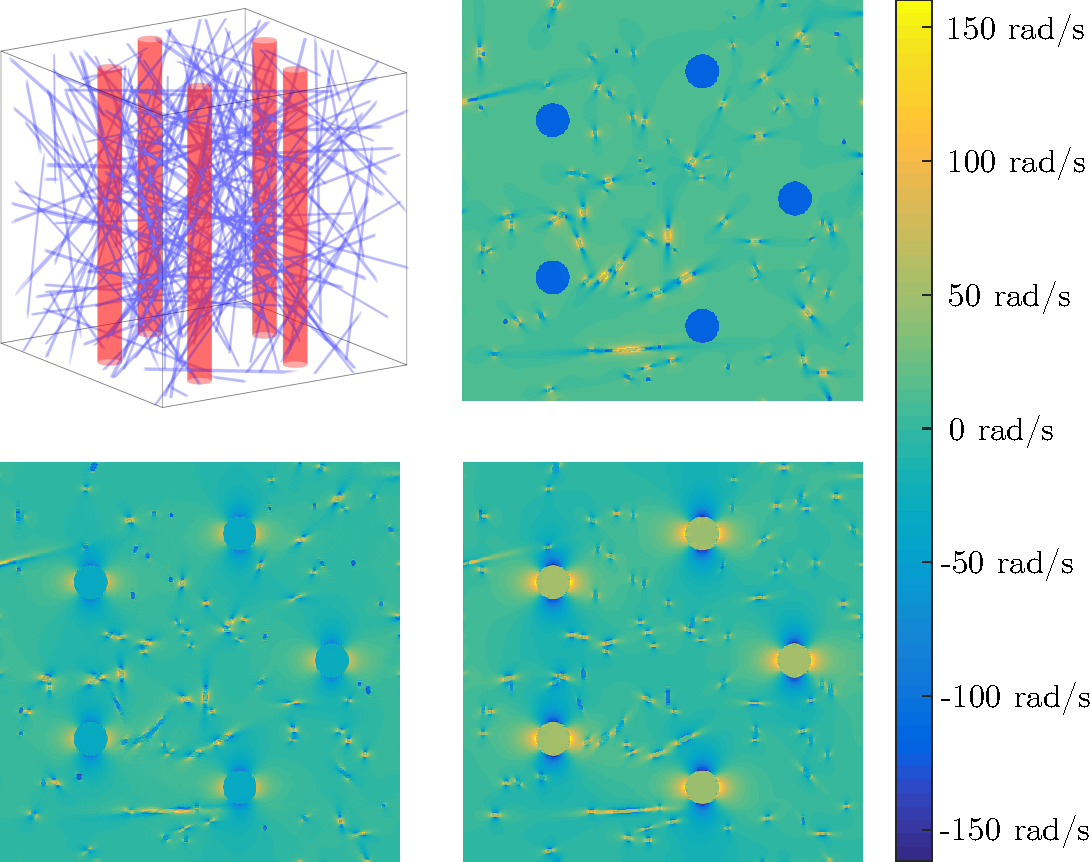
\includegraphics[keepaspectratio=true,width=\textwidth]{spin_echo/voxelgeo_domega_2x2}
    \caption{ The top-left figure shows an example voxel geometry.
      The $3\times 3\times \SI{3}{\milli\meter^3}$
      voxel is populated with an
      isotropic vascular bed and $L=5$ anisotropic large vessels in
      the $z$-direction. The total volume occupied by the blood
      vessels is determined by the blood volume fraction BVF. The
      relative fraction of blood contained in the isotropic vascular
      bed is determined by the isotropic relative blood volume
      fraction iRBVF, and the amount of blood contained in the
      anisotropic vessels is then $\text{aRBVF} = 1 - \text{iRBVF}$.
      The magnetic field generated by this configuration is computed
      by the convolution of the susceptibility map with the unit
      dipole kernel. Example cross-sections of the frequency shift
      map $\delta\omega$ are shown for $\alpha = 0\degree$ (top
      right), $45 \degree$ (bottom left), and $90 \degree$ (bottom
      right).  It can be easily observed that near large vessels, the
      resonance frequency (i.e. the magnetic field) remains locally
      relatively constant compared to the resonance frequency near
      small vessels, which changes rapidly over short distances.  Note
      also the increase in strength and range of inhomogeneities
      around the large anisotropic vessels as $\alpha$ increases,
      introducing the dependence on the angle $\alpha$ into the
      simulations.}
    \label{fig:geometry}
    \end{minipage}
\end{figure}

\clearpage
\begin{figure}[H]
\centering
\begin{minipage}{1.0\textwidth}

\centering
%\begin{minipage}{0.7\textwidth}
\begin{minipage}{1.0\textwidth}
\begin{algorithm}[H]
\setstretch{2.0}
\fontsize{16}{16}
\begin{algorithmic}[1]
    \algsetup{linenosize=\LARGE}
    \algsetup{indent=3em}
    \vspace{0.25cm}
    \STATE \text{\LARGE{}Initialize:} $\Mxy_0 \coloneqq i$,
    $\Delta t \coloneqq \text{TE}/30$, $k \coloneqq 0$

    \WHILE{ $k \Delta t < \text{TE}$ }
    
    \STATE $\Mxy_{k+\frac{1}{2}} \coloneqq 
    e^{-\CDecay(\v{x}) \Delta t} \, \Mxy_k$
    %\COMMENT{$\Delta t \rightarrow \Delta t/2$}

    \STATE $\Mxy_{k+1} \coloneqq 
    \Phi(\v{x},\Delta t) \conv \Mxy_{k+\frac{1}{2}}$
    %\COMMENT{$\Mxy_{k+1} \rightarrow \Mxy_{k+\frac{1}{2}}$}

    %\STATE \Comment{$\Mxy_{k+1} \coloneqq
    %e^{-\CDecay(\v{x}) \Delta t/2} \Mxy_{k+\frac{1}{2}}$}

    \IF{ $(k+1) \Delta t = \text{TE}/2$ }
    \STATE $\Mxy_{k+1} \coloneqq \conj{\Mxy}_{k+1}$
    \ENDIF
    
    \STATE $k \coloneqq k + 1$
    
    \ENDWHILE
    
    \STATE $S(\text{TE}) \coloneqq \int \Mxy_k \, d^3\v{x}$
\end{algorithmic}
\captionsetup{strut=off}
\caption*{\Large{}\textbf{Magnetization Propagation Algorithm}}
\end{algorithm}
\end{minipage}

%\captionsetup{font=small,skip=0pt}
\addtocounter{figure}{-1} %Want this to be labelled as the first Algorithm
\renewcommand{\figurename}{Algorithm}
\caption{Magnetization propagation algorithm used to simulate the signal
    $S(\text{TE})$ for a given set of free parameters 
    $\text{CA}_{\text{PEAK}}$, BVF, iBVF, and $L$. 
    All four free parameters are encoded solely in the complex decay rate 
    $\CDecay(\v{x})$; the rest of the algorithm does not depend on them.
    The notation $\Mxy_\nu$ is shorthand for 
    $\Mxy(\v{x},\nu \Delta t)$ throughout the algorithm.
    If the $\mathcal{O}(\Delta t^3)$ order evolution 
    equation \eqref{EvolSplit_Order3} were used instead,
    line 3 should be modified to decay for only a half time step $\Delta t/2$,
    line 4 should perform the Gaussian convolution in-place,
    and an extra line should be added directly following the convolution which
    decays for another half time step $\Delta t/2$.}
    \label{fig:algorithm1}
\end{minipage}
\end{figure}

\clearpage
\begin{figure}[H]
\centering
\begin{minipage}{1.0\textwidth}
    \centering
    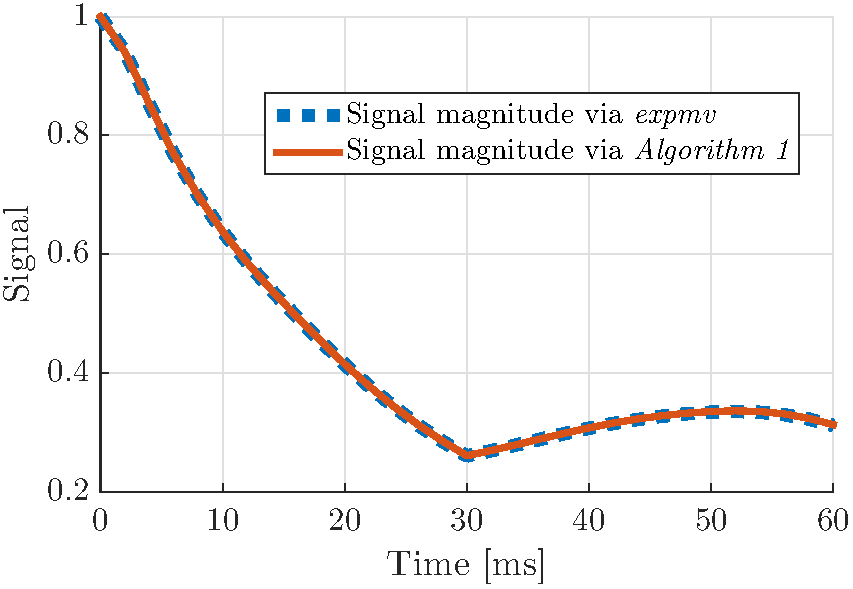
\includegraphics[keepaspectratio=true,width=1.0\textwidth]{spin_echo/SE_Signal_vs_Time_ConvDiff_vs_Expmv}
    \caption{Comparison between solving the Bloch-Torrey equation
          exactly using the method of lines in conjunction with
          Higham's \textit{expmv}
          integrator~\cite{al-mohy_computing_2011}, and solving the
          Bloch-Torrey equation approximately using the two-step
          approximate solution as described in
          Algorithm~\ref{fig:algorithm1}. The signal decay through
          time calculation shows strong agreement between the two
          methods, with error values of 0.064\% +/- 0.045\%; the
          maximum error value of 0.14\% occurs at $\unit[60]{ms}$.}
    \label{fig:comparison}
\end{minipage}
\end{figure}

\end{document}
